\section{Methods}

\subsection{Knowledge Graph Language Model}

% \frame{
%     \frametitle{The Knowledge Graph Language Model (KGLM): High-level overview}
%     \begin{itemize}
%         \item Uses a task-specific knowledge augmentation strategy for the task of language modelling using a dynamically updated local knowledge graph \cite{Logan2019BaracksModeling}.
%         \begin{itemize}
%             \item The KGLM uses the LKG to select and copy relevant information using a copy mechanism \cite{Gu2016IncorporatingLearning, Gulcehre2016PointingWords}
%             \item The local knowledge graph consists of the entities already seen in the context with their related entities and the associated relation-type.
%         \end{itemize}
%         \item Maintains two different, but not necessarily disjoint vocabularies:
%         \begin{itemize}
%             \item One related to the "background LM"
%             \item One related to the aliases of the entities in the knowledge graph
%         \end{itemize}
%         \item An example is shown on the Slide 16.
%     \end{itemize} 
% }

\frame{
    \frametitle{The KGLM: Wikidata as a Knowledge Graph}
    \begin{columns}
    \begin{column}[T]{0.5\textwidth}
        \begin{figure}
            \centering
            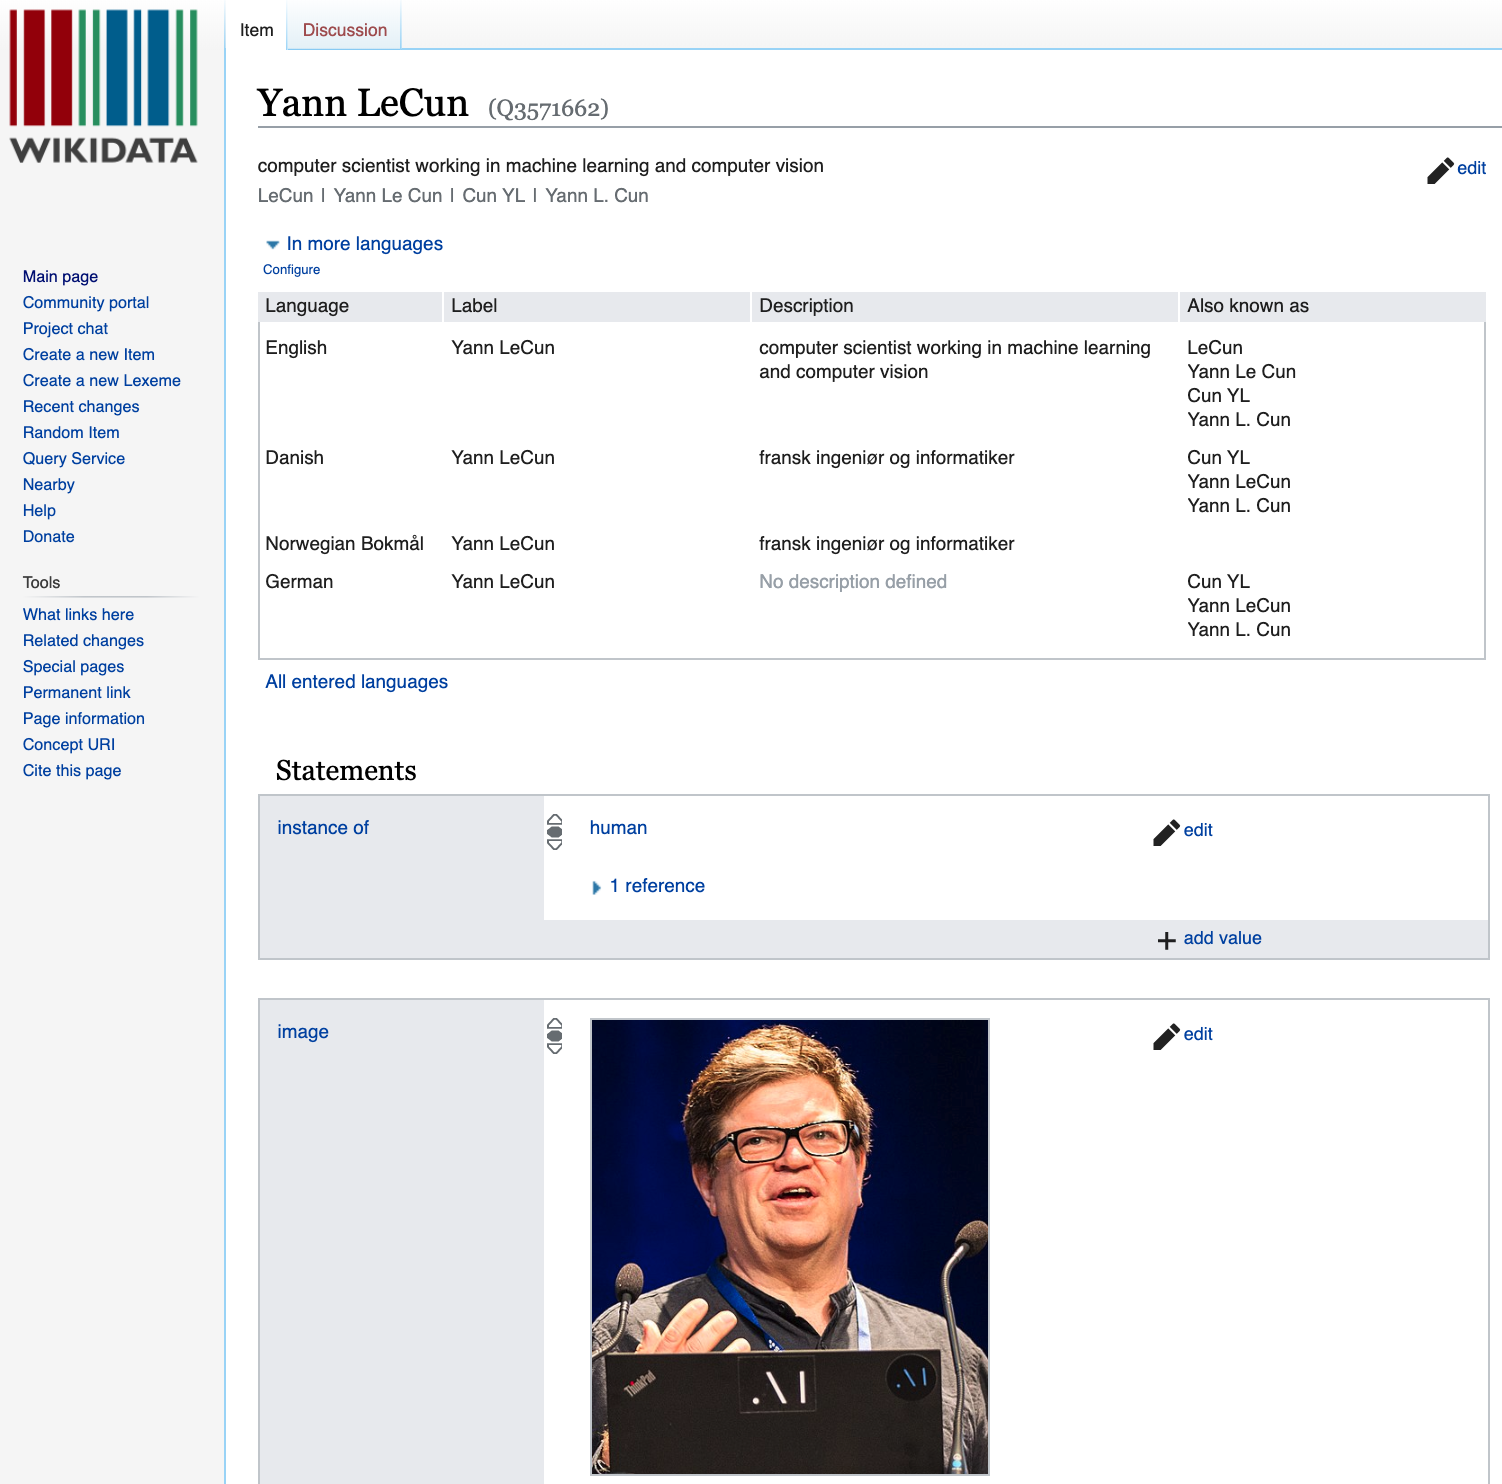
\includegraphics[height=0.8\textheight]{graphics/kglm/wikidata/wikidata_yann_lecun.png}
        \end{figure}
    \end{column}
    \begin{column}[T]{0.5\textwidth}
        \begin{figure}
            \centering
            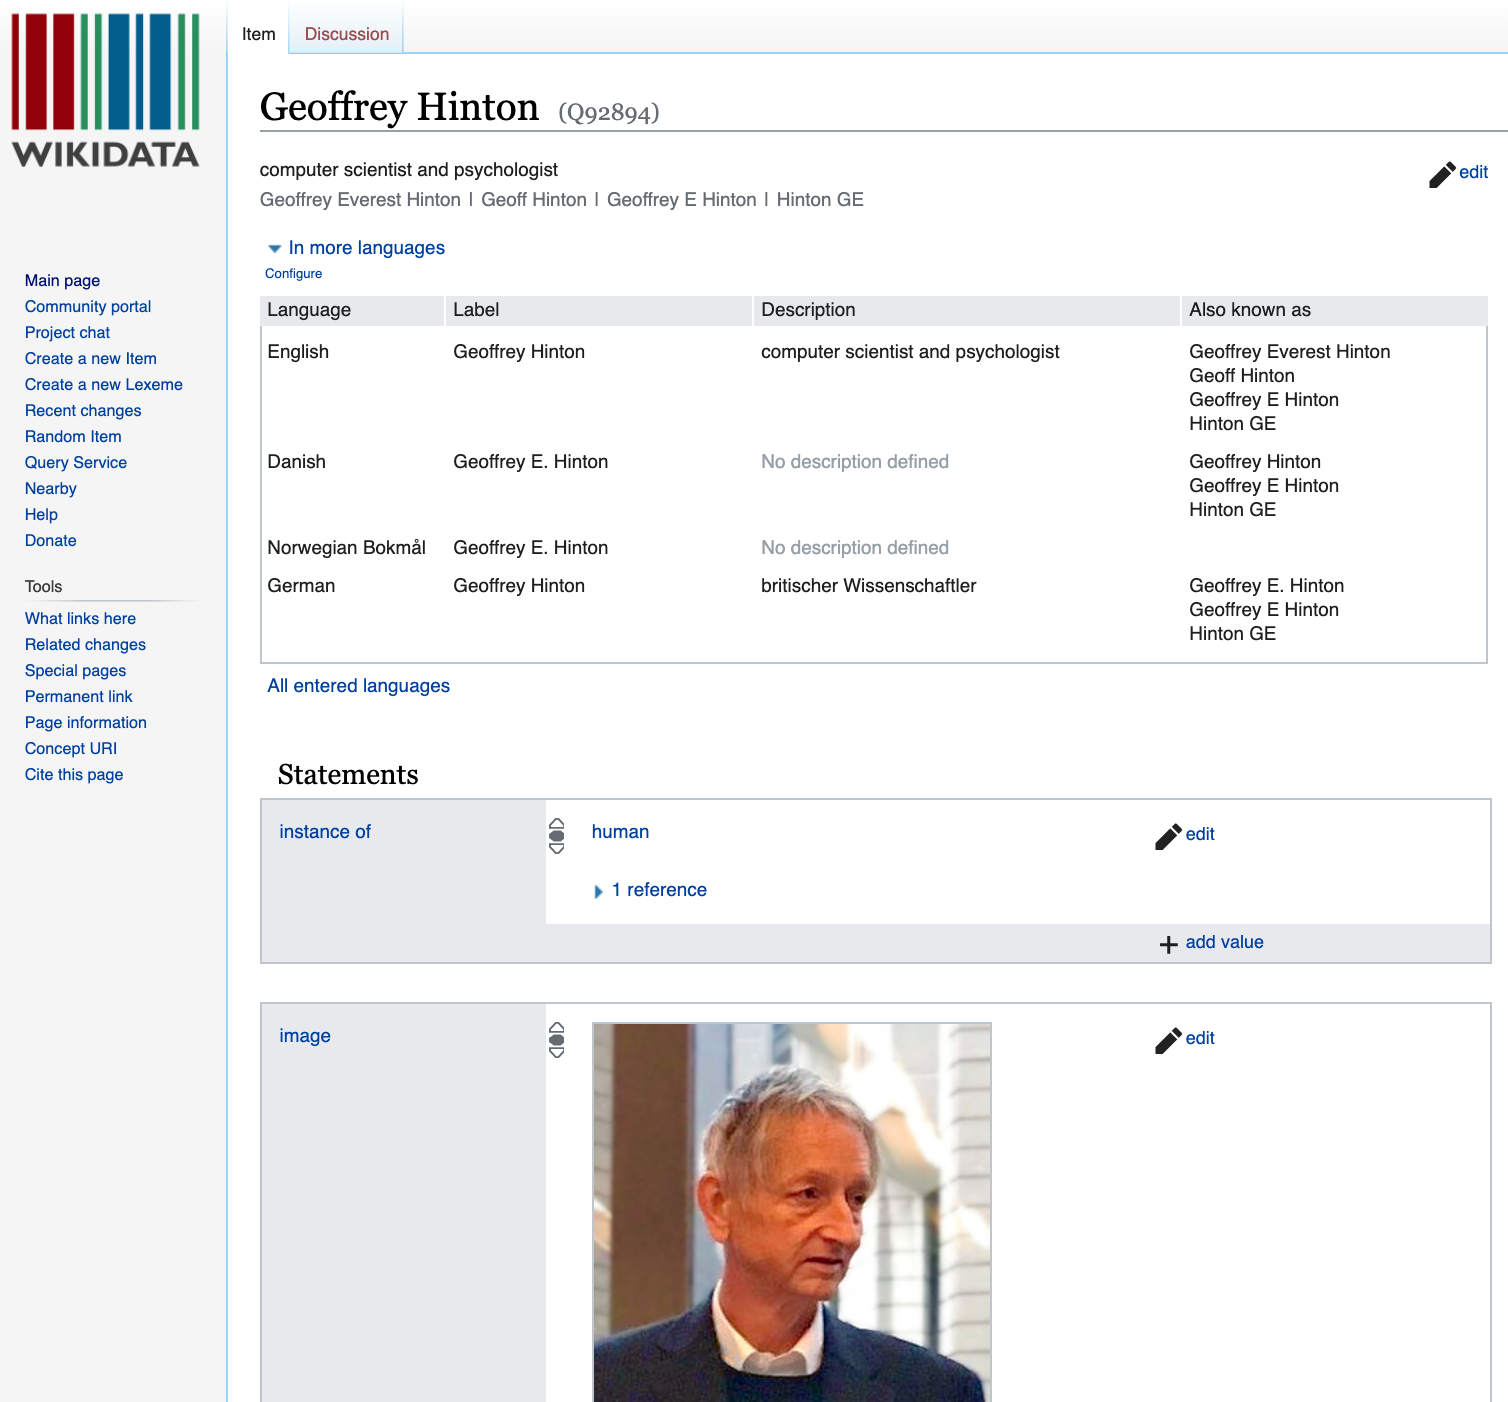
\includegraphics[height=0.8\textheight]{graphics/kglm/wikidata/wikidata_geoffrey_hinton.png}
        \end{figure}
    \end{column}
    \end{columns}
}

\frame{
    \frametitle{Delineation of the KGLM: Conceptual walk-through}
    \begin{figure}[T]
        \centering
        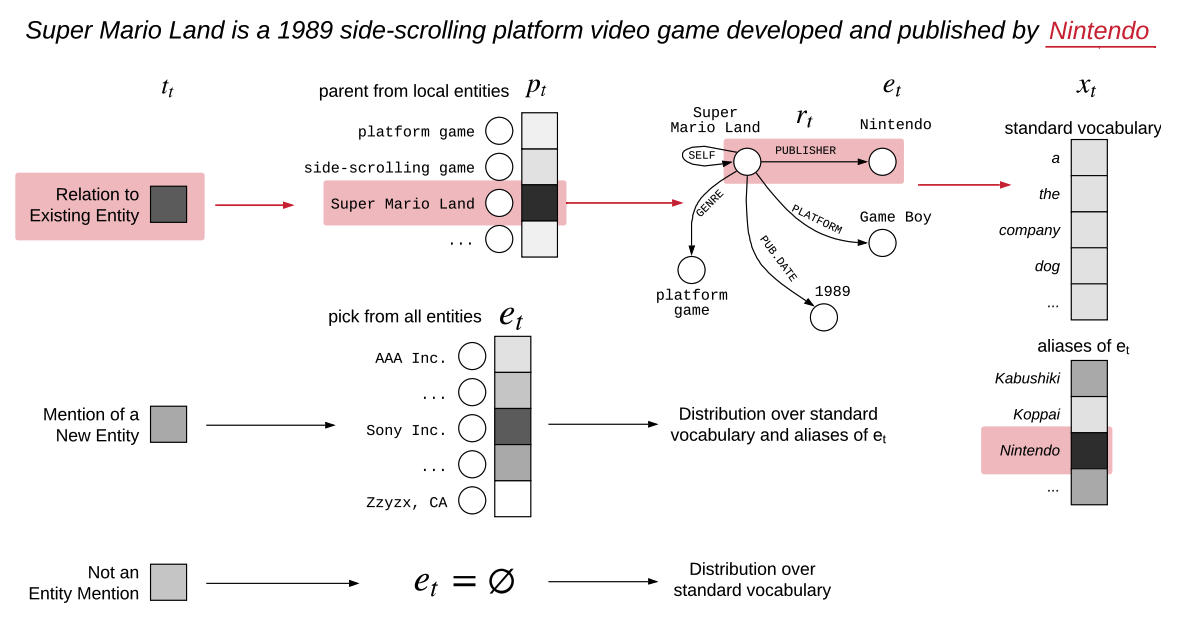
\includegraphics[width=0.8\textwidth]{graphics/kglm/generative_process/kglm_model.png}
    \end{figure}
    {\tiny Courtesy of \cite{Logan2019BaracksModeling}}
}


\frame{
    \frametitle{Delineation of the KGLM: Example Annotation}
    \begin{figure}[T]
        \centering
        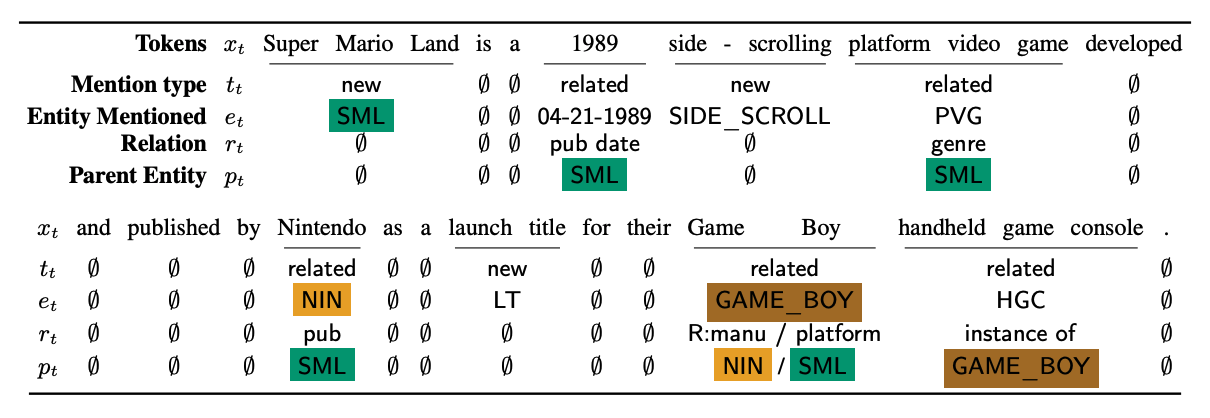
\includegraphics[width=0.8\textwidth]{graphics/kglm/generative_process/kglm_generative.png}
    \end{figure}
    {\tiny Courtesy of \cite{Logan2019BaracksModeling}}
}



\frame{
    \frametitle{Training the KGLM I: Objective}
    The objective minimised is the negative log-likelihood of the joint probability over both tokens and entities conditioned on the previous tokens and entities for all previous time-steps:
    \begin{equation*}
        \mathcal{L_{\mathrm{KGLM}}}\qty(\theta) = - \sum_t \log\, p(x_t , \Ents_t | x_1^{t-1}, \Ents_1^{t-1}; \theta) \tag{KGLM Objective}
    \end{equation*}
    where $\theta$ is the set of model parameters.\\
    Under training we observe all random variable $\rightarrow$ gradient-based optimisation \Smiley{}
}
\frame{
    \frametitle{Inference using the KGLM: How to predict the next-token at inference?}
    \textbf{Issues:}
    \begin{itemize}
        \item We need to marginalise the joint probability over everything except the tokens.
        \item Marginalisation is intractable due to combinatorial number of possible annotations.
    \end{itemize}
    \textbf{Solution:}
    Importance sampling \Smiley{}
        \begin{equation}\label{eq:KGLM_inference}
            \begin{split}
                p(\xxx) &= \sum_{\Ents} p(\xxx,\Ents) = \sum_{\Ents} \dfrac{p(\xxx, \Ents)}{q(\Ents | \xxx)} \, q(\Ents | \xxx) \\
                        & \approx \dfrac{1}{N} \sum_{\Ents \sim q} \dfrac{p(\xxx, \Ents)}{q(\Ents | \xxx)} 
            \end{split}
            \tag{KGLM Marginalisation}
        \end{equation}
    where $N$ is the number of drawn importance samples and $q$ a discriminative version of the KGLM is learned to estimate $q(\Ents | \xxx)$ to make annotations for the generative version.
        
    }

\subsection{KnowBERT}

\frame{
    \frametitle{KnowBERT: a knowledge enhancing overview}
     \begin{figure}[T]
    \centering
    \begin{tikzpicture}
    \node (BERT) at (-4.5, 0) {
\includegraphics[height=1.5cm]{graphics/auxillary/BERT_transparent.png}};
    \node (KnowBERT) at (4, 0) {
\includegraphics[height=1.5cm]{graphics/auxillary/knowbert.png}};
    \draw[-stealth] (BERT) -- (KnowBERT) node[above, midway] {\colbf{KAR}};
    \end{tikzpicture}
    \end{figure}
    \vspace{-0.85cm}
    {\footnotesize
    \begin{columns}
    \begin{column}[T]{0.5\textwidth}
    {\color{DTU_orange}\rule{\linewidth}{3pt}
    Pre-trained Model (BERT)
    \rule{\textwidth}{3pt}}
    \vspace{-0.5cm}
    \begin{itemize}
        \item Creates contextual word representations based on bi-directional LM.
        \item Pre-trained using two objectives:
        \begin{itemize}
            \item Masked Language Modelling (MLM)
            \item Next-Sentence Prediction (NSP)
        \end{itemize}
    \end{itemize}
    \end{column}
    \begin{column}[T]{0.5\textwidth}
    {\color{DTU_red}\rule{\linewidth}{3pt}
    Knowledge, Attention, and Re-contextualisation \hfill (KAR) \rule{\textwidth}{3pt}}
    \vspace{-0.5cm}
    \begin{itemize}
        \item Idea is to solder a KB between parts of BERT.
        \item In this work we focus on two KBs:
        \begin{itemize}
            \item Wikipedia where entity embeddings are learned per article
            \item WordNet is a lexical database of semantic relations between words in more than 200 languages. It consists of synsets and lemmas.
        \end{itemize}
    \end{itemize}
    \end{column}
    \end{columns}
    }
}

\frame{
    \frametitle{KnowBERT: Knowledge Base requirements}
    \begin{columns}
    \begin{column}[T]{0.5\textwidth}
    {\color{DTU_blue}\rule{\linewidth}{3pt}
    \footnotesize Knowledge Base (KB) - Definition \hfill\rule{\linewidth}{3pt}}
    \vspace{-1cm}
    \begin{figure}[T]
        \centering
        \begin{tikzpicture}
        \node[rotate=30] (0,0) {
\includegraphics[width=0.4\textwidth]{graphics/auxillary/we_got_this.jpeg}};
        \end{tikzpicture}
    \end{figure}
    \vspace{-0.9cm}
    {\footnotesize 
    .. we need to be able to create a semantic space mathematically by embedding a set of entities (and potentially relations)
    }
    \end{column}
    \begin{column}[T]{0.5\textwidth}
    \footnotesize
    {\color{DTU_yellow}\rule{\linewidth}{3pt}
    Candidate Mention Selector \hfill\rule{\linewidth}{3pt}}
        In addition, the KBs are accompanied by a candidate mention selector which generates a maximum of $C$ candidate spans.  For each of the $C$ candidate (subscript $m$) a list of $K$ candidate entities are extracted from the KB so that
        \begin{equation}\label{eq:KB}
            \begin{split}
                \mathcal{C} = \left\{ [\mathrm{start}_m,\mathrm{end}_m] \right.,& [e_{m,1},e_{m,2},...,e_{m,K}]\\
                 ,& \left.[p_{m,1}, p_{m,2}, ..., p_{m,K}] \right\} 
            \end{split}
        \end{equation}
        where the start$_m$ and end$_m$ refers to the indices of the text piece $m$, and $e_{m,k}$ is the $k$'th entity in the KB related to candidate span number $m$. \\ 
        The final vector contains the prior probabilities, $p_{m,k}$, which has been proven effective in the entity linking \cite{Ganea2017DeepAttention}.
    \end{column}
    \end{columns}
}

\frame{
    \frametitle{KnowBERT: Knowledge, Attention and Re-contextualisation (KAR)}
    \begin{columns}
    \begin{column}[T]{0.75\textwidth}
    \begin{figure}
        \centering
        \includegraphics[width=0.88\textwidth]{graphics/kb/knowbert_KAR.pdf}
    \end{figure}
    \end{column}
    \begin{column}[T]{0.35\textwidth}
        {\footnotesize 
        \begin{itemize}
            \item The \textcolor{DTU_orange}{\textbf{BERT}} encoders are used to make contextualised word representations
            \item The \colbf{KAR} mechanism is intended to handle the incorporation of external knowledge
            \item Based on the input sentence \textit{Kobe Bryant is ...}, the model creates a list of \textcolor{DTU_yellow}{\textbf{Mention Spans}} which are sub-strings of the entire sequence, e.g. \textit{Kobe}, \textit{Kobe Bryant}. Each of these has associated entities in the given KBs.
        \end{itemize}
        }
    \end{column}
    \end{columns}
}

\frame{
    \frametitle{KnowBERT: The candidate selectors and entity linking}
    \begin{figure}[t!]
        \centering
        \includegraphics[width=0.6\textwidth]{graphics/kb/knowbert_mention-span-generation.pdf}
    \end{figure}
    \vspace{-0.8cm}
    \begin{columns}
    \begin{column}[T]{0.5\textwidth}
        \begin{figure}[t!]
            \centering
            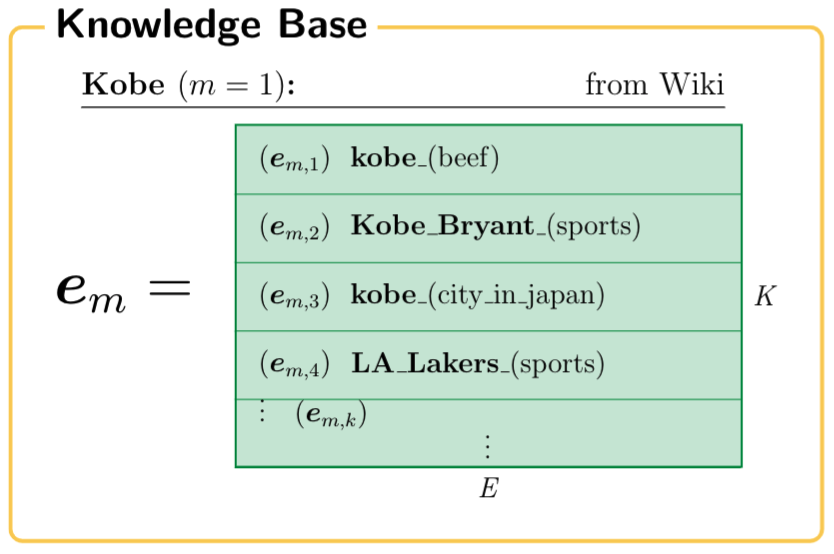
\includegraphics[width=0.6\textwidth]{graphics/kb/knowbert_mention_spans.png}
        \end{figure}
    \end{column}
    \begin{column}[T]{0.5\textwidth}
            \begin{figure}[t!]
            \centering
            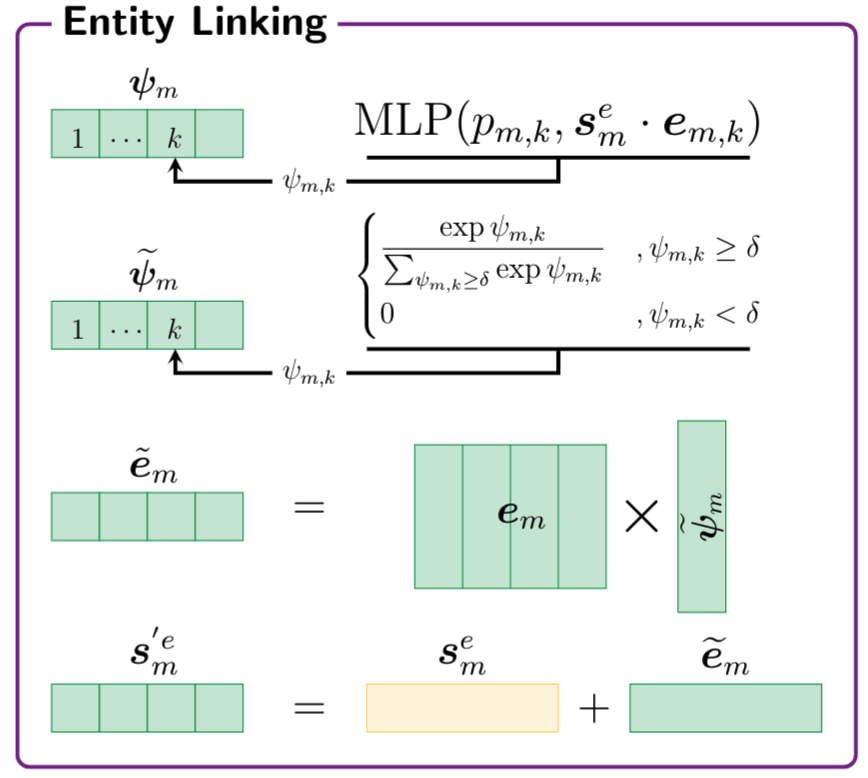
\includegraphics[width=0.5\textwidth]{graphics/kb/knowbert_entity_linking.png}
            \end{figure}
    \end{column}
    \end{columns}
}

\frame{
    \frametitle{KnowBERT: Re-contextualisation}
    \vspace{-0.5cm}
    \begin{figure}[t!]
        \centering
        \includegraphics[width=0.7\textwidth]{graphics/kb/Knowbert_KAR_mechanism.pdf}
    \end{figure}
    \vspace{-0.4cm}
    {\footnotesize
    \begin{columns}
    \begin{column}[T]{0.5\textwidth}
        {\color{DTU_red}\rule{\linewidth}{3pt}
        Multi-Headed Word-to-Entity (W2E) Attention \rule{\textwidth}{3pt}}
        %\vspace{-0.5cm}
        \begin{equation}
        \HHH_i^{'\mathrm{proj}} = \mathrm{MLP}(\mathrm{MHA}(\HHH_i^{\mathrm{proj}}, \SSS^{'e}, \SSS^{'e}))
        \tag{W2E}
        \end{equation}
        \vspace{-0.4cm}
        \begin{itemize}
            \item Allows each word in the input sentence to attend to mention spans.
            \item Peters et al. found an MLP with 1024 hidden units and 4 attention heads to be sufficient.
        \end{itemize}
    \end{column}
    \begin{column}[T]{0.5\textwidth}
        {\color{DTU_orange}\rule{\linewidth}{3pt}
        Re-contextualisation \rule{\textwidth}{3pt}}
        %\vspace{-0.4cm}
        \begin{equation}\label{eq:KG_to_BERT_projection_eq7}
            \HHH_i^{'} = \HHH_i^{'\mathrm{proj}} \WWW_2^{\mathrm{proj}} + \bbb_2^{\mathrm{proj}} + \HHH_i \tag{$\rightarrow$ BERT} 
        \end{equation}
        \vspace{-0.4cm}
        \begin{itemize}
            \item $\WWW_2^{\mathrm{proj}}$ initialised as the inverse of the learned projection to entity space, i.e., $(\WWW_1^{\mathrm{proj}})^{-1}$ to promote alignment between the contextual word representations and the entity vectors.
        \end{itemize}
    \end{column}
    \end{columns}
    }
}

\subsection{Implementation}

\frame{
    \frametitle{Allennlp}
    \begin{columns}
    \begin{column}[T]{0.5\textwidth}
        \begin{figure}
            \centering
            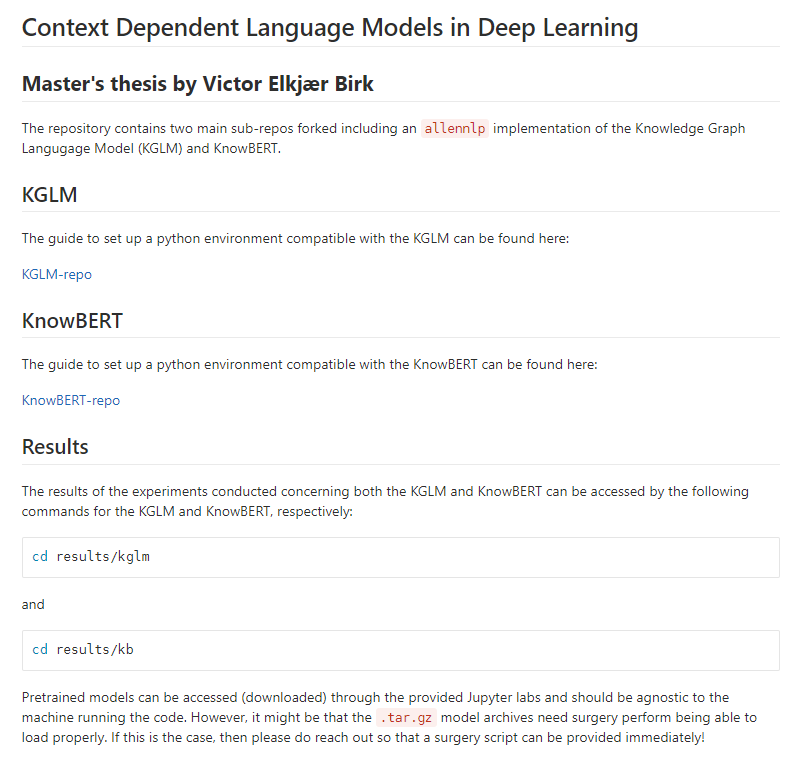
\includegraphics[height=0.9\textheight]{graphics/auxillary/gitlab_snippet.png}
        \end{figure}
    \end{column}
    \begin{column}[T]{0.5\textwidth}
        \begin{figure}
            \centering
            
\includegraphics[height=0.4\textheight]{graphics/auxillary/allenai_logo.png}
        \end{figure}
        \href{https://gitlab.gbar.dtu.dk/context-dependent-language-models/context-dependent-language-models}{\textbf{GitLab-repo can be accessed here}}
    \end{column}
    \end{columns}
}